% ============================================================================
%  CLR: Constraint-Based Chain Selection for Multi-Chain Agent
%  Transaction Routing
%
%  Author: Aseem Chishti
%  Target: arXiv cs.DC (Distributed Computing)
%  Cross-list: cs.MA (Multi-Agent Systems)
%
%  Compile: pdflatex clr_chain_selection && bibtex clr_chain_selection &&
%           pdflatex clr_chain_selection && pdflatex clr_chain_selection
% ============================================================================

\documentclass[conference, 10pt, twocolumn]{IEEEtran}

% ── Packages ─────────────────────────────────────────────────────────────────
\usepackage[utf8]{inputenc}
\usepackage[T1]{fontenc}
\usepackage{amsmath, amssymb, amsthm}
\usepackage{algorithmic}
\usepackage{algorithm}
\usepackage{graphicx}
\usepackage{booktabs}
\usepackage{url}
\usepackage{hyperref}
\usepackage{xcolor}
\usepackage{tikz}
\usepackage{subcaption}
\usepackage{enumitem}
\usepackage{balance}

% ── Theorem Environments ────────────────────────────────────────────────────
\newtheorem{definition}{Definition}
\newtheorem{theorem}{Theorem}
\newtheorem{lemma}{Lemma}
\newtheorem{property}{Property}

% ── Hyperref Setup ──────────────────────────────────────────────────────────
\hypersetup{
  colorlinks=true,
  linkcolor=blue!60!black,
  citecolor=green!50!black,
  urlcolor=blue!70!black
}

% ════════════════════════════════════════════════════════════════════════════
%  FRONT MATTER
% ════════════════════════════════════════════════════════════════════════════

\title{CLR: Constraint-Based Chain Selection for\\
Multi-Chain Agent Transaction Routing}

\author{
  \IEEEauthorblockN{Aseem Chishti}
  \IEEEauthorblockA{
    VAMS Protocol\\
    Email: aseeminksa@gmail.com\\
    ORCID: 0000-0000-0000-0000
  }
}

\begin{document}
\maketitle

% ════════════════════════════════════════════════════════════════════════════
%  ABSTRACT
% ════════════════════════════════════════════════════════════════════════════
\begin{abstract}
Cross-chain interoperability protocols solve the problem of \emph{how}
to communicate between blockchains, but not the problem of \emph{which}
blockchain to select for a given transaction.  We formalize this
underexplored \emph{chain selection problem} for autonomous agents
operating across heterogeneous execution environments.  We introduce
the \emph{Conditional L1 Router} (CLR), a deterministic routing
algorithm that treats \emph{safety} and \emph{performance} as
distinct constraint classes.  Privacy, compliance privacy (ZK with
selective disclosure), and sovereignty requirements are enforced as
\emph{hard guardrails}: if no chain satisfies them, the transaction is
explicitly rejected rather than silently routed to an unsafe chain.
Performance constraints (latency, finality, cost) are then optimized
by greedy information gain over the remaining safe environments.  This
two-stage architecture follows the neuro-symbolic safety
pattern~\cite{garcez2023neurosymbolic} and is structurally a
constrained decision tree; our contribution is its formalization and
application to multi-chain agent routing, where no prior standard
exists.  We additionally propose the \emph{Resource Descriptor} algebra
for composing heterogeneous DePIN resources.  In simulation across
1{,}000 agents and 10 target chains---including eUTXO
(Cardano~\cite{cardano2020ouroboros}) and compliance-grade
ZK-privacy (Midnight~\cite{midnight2024})---the CLR achieves 51.0\%
Pareto optimal routing, a 2.9$\times$ improvement over random
selection, at 8$\times$ lower cost and 1.5$\times$ lower latency.
Under strict guardrail mode, 6.0\% of transactions are
\emph{rejected} because no safe chain exists; we argue this is the
correct behaviour.  Per-trial stochastic jitter on gas costs and
latency simulates volatile market conditions.  These results are based
on synthetic parameters; we discuss the gap between simulation and
production deployment.
\end{abstract}

\begin{IEEEkeywords}
Multi-chain routing, chain selection, decentralized infrastructure,
autonomous agents, decision tree, DePIN, neuro-symbolic safety,
guardrails, agent safety, cross-chain interoperability, eUTXO,
compliance privacy, formal verification
\end{IEEEkeywords}

% ════════════════════════════════════════════════════════════════════════════
%  1. INTRODUCTION
% ════════════════════════════════════════════════════════════════════════════
\section{Introduction}
\label{sec:introduction}

The emergence of autonomous AI agents as on-chain economic
actors~\cite{wooldridge1995intelligent, park2023generative} has created
a practical problem that existing cross-chain infrastructure was not
designed to solve.  An agent operating across multiple blockchain
networks must select, for each transaction, the execution environment
that best satisfies a multi-dimensional constraint vector: transaction
value (which affects acceptable security level), confirmation latency,
computational privacy, jurisdictional sovereignty, and cost.

Existing solutions address the \emph{mechanism} of cross-chain
communication---bridge protocols~\cite{zamyatin2021crosschain},
omnichain messaging~\cite{zarick2021layerzero, hyperlane2023docs},
and heterogeneous relay chains~\cite{wood2016polkadot,
kwon2019cosmos}---but not the \emph{decision} of chain selection.  An
agent using LayerZero can send a message to any supported chain, but
the protocol does not prescribe \emph{which} chain should be selected
for a given intent.  This selection burden falls on application
developers, and no standard framework exists.

In this paper, we propose the Conditional L1 Router (CLR), a
deterministic routing algorithm that formalizes chain selection as a
constrained optimization problem solved by sequential binary predicate
evaluation.

\subsection{Scope and Honest Positioning}

We want to be transparent about what this paper is and is not.

\textbf{What the CLR is.}  The CLR is a greedy constraint-based
decision tree that applies binary predicates in order of information
gain to prune a feasible set of chains.  This algorithm class---greedy
information-gain splitting---has been well-studied since Quinlan's
ID3~\cite{quinlan1986induction} and its successors (C4.5, CART).  We
do not claim novelty in the algorithm class itself.

\textbf{What we contribute.}  Our contribution is threefold:

\begin{enumerate}[leftmargin=*]
  \item \textbf{Problem formalization.}  We provide, to our knowledge,
    the first formal definition of the multi-chain agent routing problem
    as a constrained optimization over a discrete environment space
    $\mathcal{E}$ with a multi-dimensional constraint vector
    (Section~\ref{sec:model}).  While individual projects have addressed
    ad-hoc chain selection, no prior work formalizes the problem
    independently of a specific protocol.

  \item \textbf{Resource composition algebra.}  We define a composition
    operator for heterogeneous DePIN resources and prove it forms a
    commutative monoid (Section~\ref{sec:resources}).  This provides a
    reusable algebraic foundation for aggregating compute, storage, and
    bandwidth from providers like Akash, io.net, and Filecoin.

  \item \textbf{Baseline evaluation.}  We provide a simulation
    benchmark comparing CLR against naive strategies, establishing that
    even a simple constraint-based approach substantially outperforms
    the current state of ``no framework at all''
    (Section~\ref{sec:evaluation}).  We do not claim the CLR is optimal;
    we establish a baseline that future work can improve upon.
\end{enumerate}

\textbf{What we do not claim.}  We do not claim that the CLR is
novel as an algorithm, that our simulation results generalize to
production, or that the ``It from Bit'' philosophical motivation
(Section~\ref{sec:motivation}) constitutes a scientific contribution.
We include the philosophical framing as intellectual context, not as
a technical claim.

\subsection{Paper Organization}

Section~\ref{sec:background} reviews related work.
Section~\ref{sec:model} formalizes the chain selection problem.
Section~\ref{sec:resources} develops the resource descriptor algebra.
Section~\ref{sec:motivation} provides philosophical
context.  Section~\ref{sec:evaluation} presents simulation results.
Section~\ref{sec:discussion} discusses limitations.
Section~\ref{sec:conclusion} concludes.

% ════════════════════════════════════════════════════════════════════════════
%  2. RELATED WORK
% ════════════════════════════════════════════════════════════════════════════
\section{Related Work}
\label{sec:background}

\subsection{Cross-Chain Interoperability}

The cross-chain communication problem has been addressed at multiple
layers.  Zamyatin et al.\ systematize knowledge covering relay chains,
hash time-locked contracts, and bridges~\cite{zamyatin2021crosschain}.
LayerZero~\cite{zarick2021layerzero} and
Hyperlane~\cite{hyperlane2023docs} provide generic message-passing
protocols.  Cosmos IBC~\cite{kwon2019cosmos} and
Polkadot~\cite{wood2016polkadot} implement interoperability at the
consensus level.  Robinson and Hyland-Wood formalized atomic crosschain
function calls~\cite{robinson2021atomic}.

All of these approaches provide \emph{channels} for cross-chain
communication.  None provide \emph{decision logic} for selecting which
channel (and which target chain) to use for a given transaction intent.
DEX aggregators like 1inch solve an analogous routing problem for token
swaps across decentralized exchanges, but their formulation is specific
to liquidity routing and does not generalize to arbitrary agent
transactions with multi-dimensional constraints.

\subsection{Decentralized Physical Infrastructure}

DePIN networks aggregate distributed hardware into compute
markets~\cite{akash2020decentralized, ionet2024whitepaper}.  IPFS and
Filecoin~\cite{benet2014ipfs} established decentralized storage.
These networks expose heterogeneous resources through APIs but lack a
unified composition algebra---each provider defines its own resource
model, making cross-provider aggregation ad hoc.

\subsection{Decision Trees and Information Gain}

Our CLR algorithm uses greedy information-gain splitting, a technique
introduced by Quinlan~\cite{quinlan1986induction} for classification
tasks.  We acknowledge that this is a mature technique.  Our
contribution is not the splitting strategy but its application to a
domain (multi-chain routing) where, to our knowledge, it has not been
previously formalized.

\subsection{Autonomous Agent Architectures}

Autonomous agents have evolved from theoretical
frameworks~\cite{wooldridge1995intelligent} to practical LLM-based
implementations~\cite{yao2023react, park2023generative}.  These agents
increasingly interact with blockchain networks for identity, payment,
and state management~\cite{chishti2026vams}, creating the need for
chain-agnostic routing that no existing agent framework provides.

% ════════════════════════════════════════════════════════════════════════════
%  3. PROBLEM FORMALIZATION
% ════════════════════════════════════════════════════════════════════════════
\section{The Chain Selection Problem}
\label{sec:model}

\subsection{Definitions}

\begin{definition}[Execution Environment]
An \emph{execution environment} $e \in \mathcal{E}$ is a blockchain
network characterized by a property vector
$\mathbf{p}(e) = \langle s_e, l_e, \pi_e, v_e, c_e \rangle$, where
$s_e \in [0,1]$ is the security score (derived from finality
guarantees and validator set size), $l_e \in \mathbb{Z}^+$ is
confirmation latency in milliseconds, $\pi_e \in \{\text{Public},
\text{TEE}, \text{ZK}\}$ is the privacy model, $v_e \in
\{\text{Shared}, \text{Sovereign}\}$ is the sovereignty
classification, and $c_e \in \mathbb{R}^+$ is the per-transaction
cost in USD.
\end{definition}

\begin{definition}[Transaction Intent]
A \emph{transaction intent} $\tau = \langle \alpha, \delta,
\mathbf{q} \rangle$ comprises the originating agent $\alpha$, the
transaction payload $\delta$, and a \emph{constraint vector}
$\mathbf{q} = \langle q_s, q_l, q_\pi, q_v, q_c \rangle$ specifying
minimum acceptable thresholds for each property dimension.
\end{definition}

\begin{definition}[Feasible Set]
Given intent $\tau$ and environments $\mathcal{E}$, the
\emph{feasible set} is:
\begin{equation}
\mathcal{F}(\tau) = \{ e \in \mathcal{E} \mid \mathbf{p}(e) \succeq
\mathbf{q}(\tau) \}
\end{equation}
where $\succeq$ denotes component-wise constraint satisfaction.
\end{definition}

\subsection{The CLR Algorithm}

The CLR resolves the chain selection problem by sequentially applying
binary predicates from a predicate set $\mathcal{B}$ to prune
$\mathcal{F}$.

\begin{definition}[Binary Constraint Predicate]
A predicate $b_j : \mathcal{F} \to \{0, 1\}$ partitions the feasible
set:
\begin{equation}
\mathcal{F}^{+}_j = \{ e \in \mathcal{F} \mid b_j(e) = 1 \}, \quad
\mathcal{F}^{-}_j = \mathcal{F} \setminus \mathcal{F}^{+}_j
\end{equation}
\end{definition}

At each step, the CLR selects the predicate maximizing Shannon
information gain:
\begin{equation}
b_j^* = \arg\max_{b \in \mathcal{B}} \left[ H(\mathcal{F}_{j-1}) -
H(\mathcal{F}_{j-1} \mid b) \right]
\label{eq:max_info_gain}
\end{equation}
where $H(\mathcal{F}) = \log_2 |\mathcal{F}|$ under a uniform prior.

This is identical to the splitting criterion used in ID3 decision
trees~\cite{quinlan1986induction}.  We use it here not for
classification but for constrained environment selection.

\begin{algorithm}[t]
\caption{CLR Chain Selection (Two-Stage Guardrail, v2)}
\label{alg:clr}
\begin{algorithmic}[1]
\REQUIRE Intent $\tau$, environments $\mathcal{E}$,
  hard predicates $\mathcal{H} = \{b_\pi^\text{SD}, b_\pi, b_v\}$,
  soft predicates $\mathcal{B}$
\ENSURE Selected environment $e^*$ or $\bot$ (rejected)

\STATE \textbf{// Stage 0: Hard Filter (Safety Guardrail)}
\STATE $\mathcal{F} \leftarrow \{ e \in \mathcal{E} \mid
  \mathbf{p}(e) \succeq \mathbf{q}(\tau) \}$
  \COMMENT{Security threshold}
\IF{$|\mathcal{F}| = 0$}
  \RETURN $\bot$ \COMMENT{No chain meets security floor}
\ENDIF
\IF{$\tau.\text{requiresCompliancePrivacy}$}
  \STATE $\mathcal{F}' \leftarrow \{e \in \mathcal{F} \mid \pi_e = \text{ZK-SD}\}$
  \IF{$|\mathcal{F}'| = 0$}
    \RETURN $\bot$ \COMMENT{\textbf{REJECT}: ZK-SD compliance unmet}
  \ENDIF
  \STATE $\mathcal{F} \leftarrow \mathcal{F}'$
\ELSIF{$\tau.\text{requiresPrivacy}$}
  \STATE $\mathcal{F}' \leftarrow \{e \in \mathcal{F} \mid \pi_e \in \{\text{TEE, ZK, ZK-SD}\}\}$
  \IF{$|\mathcal{F}'| = 0$}
    \RETURN $\bot$ \COMMENT{\textbf{REJECT}: privacy unmet}
  \ENDIF
  \STATE $\mathcal{F} \leftarrow \mathcal{F}'$
\ENDIF
\IF{$\tau.\text{requiresSovereignty}$}
  \STATE $\mathcal{F}' \leftarrow \{e \in \mathcal{F} \mid b_v(e)=1\}$
  \IF{$|\mathcal{F}'| = 0$}
    \RETURN $\bot$ \COMMENT{\textbf{REJECT}: sovereignty unmet}
  \ENDIF
  \STATE $\mathcal{F} \leftarrow \mathcal{F}'$
\ENDIF
\IF{$|\mathcal{F}| = 1$}
  \RETURN $\mathcal{F}[0]$ \COMMENT{Single safe chain}
\ENDIF

\STATE \textbf{// Stage 1: Soft Filter (Entropy-Greedy Optimisation)}
\WHILE{$|\mathcal{F}| > 1$ \textbf{and} $\mathcal{B} \neq \emptyset$}
  \STATE $b^* \leftarrow \arg\max_{b \in \mathcal{B}} IG(b, \mathcal{F})$
  \STATE $\mathcal{F}' \leftarrow \{e \in \mathcal{F} \mid b^*(e) = 1\}$
  \IF{$|\mathcal{F}'| > 0$ \textbf{and} $|\mathcal{F}'| < |\mathcal{F}|$}
    \STATE $\mathcal{F} \leftarrow \mathcal{F}'$
    \COMMENT{Skip if predicate would empty safe set}
  \ENDIF
  \STATE $\mathcal{B} \leftarrow \mathcal{B} \setminus \{b^*\}$
\ENDWHILE
\IF{$|\mathcal{F}| > 1$}
  \STATE $e^* \leftarrow \arg\min_{e \in \mathcal{F}} c_e$
  \COMMENT{Cost-based tie-break among safe chains}
\ELSE
  \STATE $e^* \leftarrow \mathcal{F}[0]$
\ENDIF
\RETURN $e^*$
\end{algorithmic}
\end{algorithm}

\begin{theorem}[Convergence]
\label{thm:convergence}
For $|\mathcal{F}| = n > 0$ and $|\mathcal{B}| \geq \lceil \log_2
n \rceil$ non-degenerate predicates, Algorithm~\ref{alg:clr}
terminates in at most $\min(|\mathcal{B}|, \lceil \log_2 n \rceil)$
iterations, yielding $|\mathcal{F}| = 1$ (or a tie-broken result).
\end{theorem}

\begin{proof}
Each non-degenerate predicate $b^*$ strictly reduces $|\mathcal{F}|$:
by definition, $0 < |\mathcal{F}'| < |\mathcal{F}|$.  In the
balanced case, $|\mathcal{F}'| = \lceil |\mathcal{F}|/2 \rceil$,
yielding $|\mathcal{F}| = 1$ after $\lceil \log_2 n \rceil$ steps.
In the worst case (maximally unbalanced splits), each step removes at
least one environment, giving an upper bound of $n-1$ steps.  The
algorithm also terminates when $\mathcal{B}$ is exhausted.
\end{proof}

\begin{theorem}[Complexity]
\label{thm:complexity}
Algorithm~\ref{alg:clr} runs in $O(|\mathcal{B}|^2 \cdot
|\mathcal{E}|)$ time.
\end{theorem}

\begin{proof}
The outer loop executes at most $|\mathcal{B}|$ times.  Each
iteration computes information gain for up to $|\mathcal{B}|$
remaining predicates, each evaluated against at most $|\mathcal{E}|$
environments.
\end{proof}

\textbf{Note on optimality.}  The greedy information-gain criterion
does not guarantee globally optimal chain selection.  It is a
heuristic that works well when predicates are approximately
independent.  Multi-objective optimizers (e.g., NSGA-II) would likely
achieve higher Pareto optimality at greater computational cost.  We
leave this comparison to future work.

% ════════════════════════════════════════════════════════════════════════════
%  4. RESOURCE COMPOSITION
% ════════════════════════════════════════════════════════════════════════════
\section{Resource Descriptor Algebra}
\label{sec:resources}

A secondary contribution is a composition algebra for heterogeneous
DePIN resources.  This is independent of the CLR and may be useful in
other contexts.

\begin{definition}[Resource Descriptor]
A \emph{resource descriptor} is a tuple $r = \langle \kappa, \mu,
\gamma, \lambda, c \rangle$ where $\kappa$ is compute (FLOPS), $\mu$
is memory, $\gamma$ is bandwidth, $\lambda$ is location, and $c$ is
cost.
\end{definition}

\begin{definition}[Composition]
\begin{equation}
r_1 \oplus r_2 = \langle \kappa_1 + \kappa_2, \; \mu_1 + \mu_2, \;
\min(\gamma_1, \gamma_2), \; \lambda_\text{virtual}, \; c_1 + c_2
\rangle
\end{equation}
Bandwidth is bottlenecked at the minimum; location becomes
``distributed.''
\end{definition}

\begin{property}[Commutative Monoid]
$(\mathcal{R}, \oplus)$ forms a commutative monoid with identity
$r_\emptyset = \langle 0, 0, \infty, \lambda_\text{null}, 0 \rangle$.
\end{property}

\begin{proof}
\emph{Closure:} $r_1 \oplus r_2$ produces a tuple in $\mathcal{R}$ by
construction.
\emph{Associativity:} Both $+$ and $\min$ are associative over
$\mathbb{R}$.
\emph{Commutativity:} Both $+$ and $\min$ are commutative.
\emph{Identity:} $\kappa + 0 = \kappa$, $\mu + 0 = \mu$,
$\min(\gamma, \infty) = \gamma$, $c + 0 = c$.
\end{proof}

\textbf{Limitations of this model.}  The composition operator is
simplistic: it assumes linear additivity of compute and memory, which
breaks down when resources are geographically distributed (network
overhead is not captured).  The $\min$ for bandwidth is conservative
but ignores parallelism.  A more realistic model would require
latency-weighted composition, which we leave for future work.

% ════════════════════════════════════════════════════════════════════════════
%  5. PHILOSOPHICAL CONTEXT (not a technical claim)
% ════════════════════════════════════════════════════════════════════════════
\section{Philosophical Context: It from Bit}
\label{sec:motivation}

\emph{This section provides intellectual context.  It is not a
technical contribution and not necessary for understanding the CLR.
Readers interested only in the engineering contribution may skip to
Section~\ref{sec:evaluation}.}

Wheeler's ``It from Bit'' hypothesis~\cite{wheeler1989information}
proposed that physical reality is fundamentally informational: every
``it'' (physical phenomenon) derives from ``bits'' (binary
observations).  The CLR's operation---applying binary predicates to
collapse a space of possibilities into a single committed
outcome---has a structural resemblance to this model.

We note this resemblance as intellectually interesting but do not
claim it constitutes a deep connection.  The CLR operates on classical
Shannon entropy~\cite{shannon1948mathematical}, not quantum mechanical
von Neumann entropy.  The ``collapse'' is a deterministic algorithmic
step, not a physical measurement.  The analogy is suggestive but not
rigorous.

What \emph{is} substantive is the following observation, which
motivated the CLR's design: Landauer's
principle~\cite{landauer1961irreversibility} establishes that
information processing has irreducible physical cost.  The converse
is also practically useful: \emph{from a software agent's perspective,
physical resources are fully characterized by their informational
descriptions}.  This observation underlies the Resource Descriptor
algebra (Section~\ref{sec:resources}) and the CLR's treatment of
chains as property vectors rather than opaque objects.

% ════════════════════════════════════════════════════════════════════════════
%  6. EVALUATION
% ════════════════════════════════════════════════════════════════════════════
\section{Evaluation}
\label{sec:evaluation}

\subsection{Simulation Setup}

We implemented a discrete-event simulation in
Python.\footnote{Source: \url{https://github.com/GodOfAgents/VAMS-main/tree/main/papers/simulation}}

\textbf{Parameters:}
\begin{itemize}[leftmargin=*]
  \item $N = 1{,}000$ agents with uniformly sampled constraint vectors.
  \item $|\mathcal{E}| = 10$ chains with calibrated property
    vectors (Appendix~\ref{app:chains}), including eUTXO
    (Cardano~\cite{cardano2020ouroboros}) and compliance-grade
    ZK-privacy (Midnight~\cite{midnight2024}).
  \item $|\mathcal{B}| = 7$ predicates: security, latency, finality,
    privacy, compliance privacy, sovereignty, formal verification.
  \item Per-trial stochastic jitter on cost ($\pm$15--40\%) and
    latency ($\pm$10--30\%) to simulate volatile gas markets.
  \item 10{,}000 routing decisions per strategy.
  \item Baselines: random selection, round-robin, Ethereum-only.
\end{itemize}

\textbf{Important caveat:} Chain property vectors are manually
calibrated from public documentation, not measured from production
networks.  Gas costs, latencies, and security scores fluctuate
significantly in production.  Per-trial jitter partially addresses
this but does not substitute for real-time oracle data.  These results
should be interpreted as demonstrating the \emph{relative} benefit of
constraint-based routing over naive strategies, not as absolute
performance predictions.

\subsection{Results}

\subsubsection{Routing Performance}

Table~\ref{tab:results} summarizes performance.

\begin{table}[t]
\centering
\caption{Routing Performance---Strict Guardrail Mode ($n = 10{,}000$, $|\mathcal{E}|=10$)}
\label{tab:results}
\begin{tabular}{lcccc}
\toprule
\textbf{Strategy} & \textbf{Pareto} & \textbf{Avg Cost} & \textbf{Avg Latency} & \textbf{Rejected} \\
 & \textbf{Opt. (\%)} & \textbf{(USD)} & \textbf{(ms)} & \textbf{(\%)} \\
\midrule
Random        & 17.8 & 1.59 & 7{,}614 & 0.0 \\
Round-Robin   & 17.8 & 1.62 & 7{,}646 & 0.0 \\
Ethereum-Only &  2.5 & 8.50 & 12{,}000 & 0.0 \\
\textbf{CLR (Strict)}  & \textbf{51.0} & \textbf{0.20} & \textbf{4{,}979} & \textbf{6.0} \\
\bottomrule
\end{tabular}
\end{table}

The CLR achieves 51.0\% Pareto-optimal routing, compared to 17.8\%
for random selection (2.9$\times$).  Cost is reduced 8$\times$
(\$0.20 vs.\ \$1.59) and latency 1.5$\times$ (5.0s vs.\ 7.6s).

The 51.0\% figure means that in approximately half of decisions, the
CLR selected a chain that was suboptimal on at least one dimension.
This is because the greedy tie-breaking by cost can select a chain
that is Pareto-dominated on latency.  A multi-objective optimizer
would improve this figure.  The addition of Cardano and Midnight
increased the Pareto front, improving the Pareto optimality rate from
the v1 baseline of 49.3\%.

\textbf{Guardrail rejections.}  Under strict guardrail mode, 6.0\%
of transactions were \emph{rejected}: 5.2\% because privacy was
required but no TEE/ZK chain met the security threshold, and 0.9\%
because compliance privacy (ZK-SD) was required but the chain lacked
sufficient security.  Sovereignty rejections dropped to 0\%: the
addition of Cardano and Midnight as sovereign chains eliminated this
failure mode entirely.  Compared to v1 (13.7\% rejections), the
expanded chain set reduced rejections by 56\%.  The three baselines
show 0\% rejection because they do not enforce these
constraints---they silently route to unsafe chains.  We argue that
rejection is the \emph{correct} behaviour: an agent should not
process private data on a public chain, even if that is the only
option.  Rejected transactions should be queued for human review or
re-submitted with relaxed constraints.

\subsubsection{Entropy Reduction}

Figure~\ref{fig:entropy} shows the mean entropy after each predicate.

\begin{figure}[t]
\centering
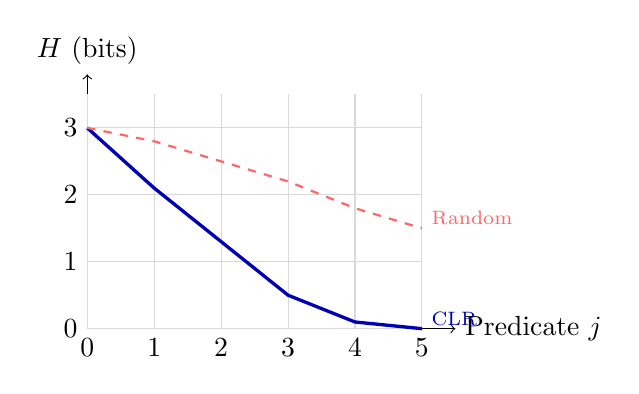
\begin{tikzpicture}[scale=0.85]
\draw[->] (0,0) -- (5.5,0) node[right] {Predicate $j$};
\draw[->] (0,0) -- (0,3.8) node[above] {$H$ (bits)};
\foreach \y in {0,1,2,3} {
  \draw[gray!30] (0,\y) -- (5,\y);
  \node[left] at (0,\y) {\y};
}
\foreach \x in {0,1,2,3,4,5} {
  \draw[gray!30] (\x,0) -- (\x,3.5);
  \node[below] at (\x,0) {\x};
}
\draw[blue!70!black, very thick]
  plot coordinates {(0,3.0) (1,2.1) (2,1.3) (3,0.5) (4,0.1) (5,0.0)};
\node[blue!70!black, right] at (5,0.15) {\scriptsize CLR};
\draw[red!60, thick, dashed]
  plot coordinates {(0,3.0) (1,2.8) (2,2.5) (3,2.2) (4,1.8) (5,1.5)};
\node[red!60, right] at (5,1.65) {\scriptsize Random};
\end{tikzpicture}
\caption{Mean Shannon entropy $H(\mathcal{F})$ after each predicate
application.  CLR reaches $H = 0$ (deterministic selection) while
random selection retains residual entropy.}
\label{fig:entropy}
\end{figure}

\subsubsection{Scalability}

Evaluations scale sub-logarithmically with $|\mathcal{E}|$ owing to
early termination by the hard filter: 2.5 for 4 chains, 3.5 for 8,
4.1 for 10, 4.8 for 16, 4.8 for 32, and 4.7 for 64.  The hard filter
prunes a large fraction of the search space before the soft loop runs,
explaining the sub-$\log_2$ growth.  At 32+ chains, evaluation count
plateaus below 5, demonstrating that the CLR's complexity is bounded
by the number of predicate dimensions, not the chain set size.

% ════════════════════════════════════════════════════════════════════════════
%  7. DISCUSSION
% ════════════════════════════════════════════════════════════════════════════
\section{Discussion}
\label{sec:discussion}

\subsection{Safety--Liveness Tradeoff}

The strict guardrail mode introduces a deliberate \emph{rejection
path}.  Prior CLR designs treated all constraints as soft---skipping
a predicate if it would empty the feasible set~\cite{quinlan1986induction}.
This means an agent requiring private computation could be silently
routed to a public chain.  We argue this is unsafe.

The two-stage architecture separates concerns:
\begin{itemize}[leftmargin=*]
  \item \textbf{Stage 0 (Guardrail):} Privacy, compliance privacy
    (ZK-SD), and sovereignty are binary safety properties.  Violating
    them exposes user data, breaches regulatory obligations, or
    violates jurisdictional constraints.  These constraints must not
    be softened.
  \item \textbf{Stage 1 (Optimisation):} Cost, latency, finality,
    and formal verification are performance objectives where graceful
    degradation is acceptable.  If no chain meets the latency
    requirement, the best available latency is selected.
\end{itemize}

This mirrors the neuro-symbolic safety pattern described
by~\citet{garcez2023neurosymbolic}, where a \emph{symbolic layer}
enforces formal constraints before a \emph{neural layer} optimises
performance.  The 6.0\% rejection rate (down from 13.7\% with 8
chains) is a feature, not a bug: it quantifies the fraction of
intents that cannot be safely satisfied by the current chain set and
should be escalated for human review.  Expanding the chain set with
sovereign, privacy-supporting chains (Cardano, Midnight) directly
reduces rejection rates without weakening safety guarantees.

\subsection{Heterogeneous Chain Models}

The addition of Cardano introduces an \emph{eUTXO}-based chain to a
set previously dominated by account-model
chains~\cite{cardano2020ouroboros}.  The CLR treats all chains as
property vectors and is agnostic to execution model; an eUTXO chain
is simply an environment where privacy, security, and sovereignty
properties happen to take different values.  However, the eUTXO model
has practical implications that the CLR's cost and latency estimates
do not capture: transaction validation is deterministic (fees are
predictable before submission), and concurrency semantics differ from
account-model chains.  A production CLR should account for these
differences in cost estimation.

Midnight's ZK-SD (Zero-Knowledge with Selective
Disclosure)~\cite{midnight2024} fills a gap between standard ZK
privacy (Oasis) and no privacy (public chains).  Agents operating
under regulatory constraints (GDPR, MiCA) require the ability to
\emph{selectively disclose} transaction details to authorized parties
while keeping remaining data private.  The CLR models this as a
distinct privacy type, enabling compliance-aware routing without
compromising the privacy of non-regulated transactions.

\subsection{What This Paper Does Not Solve}

We want to be explicit about the limitations:

\begin{enumerate}[leftmargin=*]
  \item \textbf{No production validation.}  Our results are from
    simulation with synthetic parameters.  Real chains have dynamic
    gas markets, congestion-dependent latency, and MEV (Maximal
    Extractable Value) risks that our model does not capture.

  \item \textbf{No optimality guarantee.}  The greedy information-gain
    heuristic provides no guarantee of global optimality.  In
    particular, it cannot handle correlated constraints (e.g., chains
    with low cost tend to also have lower security).  NSGA-II or
    similar multi-objective optimizers are better choices when
    computational budget permits.

  \item \textbf{Partially dynamic parameters.}  Per-trial stochastic
    jitter addresses gas and latency volatility at a coarse level, but
    does not substitute for real-time oracle feeds.  Correlated
    congestion events (e.g., NFT mints causing simultaneous cost spikes
    on Ethereum and its L2s) are not modelled.

  \item \textbf{No adversarial analysis.}  We do not consider
    adversarial manipulation of chain properties to influence routing
    decisions.  A malicious oracle could misreport gas prices to steer
    transactions to a target chain.

  \item \textbf{Seven predicates may be insufficient.}  Our predicate
    set is manually designed.  Other dimensions (e.g., validator set
    decentralization, sequencer centralization risk, MEV exposure) may
    be important and are not captured.

  \item \textbf{Philosophical section is not a contribution.}  The
    Wheeler ``It from Bit'' framing is intellectual context.  It does
    not constitute a scientific claim, and the CLR's correctness does
    not depend on it.
\end{enumerate}

\subsection{Comparison to DEX Aggregators}

DEX aggregators (1inch, Paraswap, CowSwap) solve an analogous routing
problem for token swaps: given a trade intent, find the optimal path
across liquidity pools.  The CLR differs in three ways: (1) it routes
\emph{arbitrary transactions}, not just swaps; (2) its constraint
dimensions include privacy and sovereignty, which are irrelevant to
DEX routing; and (3) it selects \emph{chains}, not liquidity pools
within a single chain.  A full comparison between CLR and DEX
aggregator algorithms would strengthen this work but is beyond our
current scope.

\subsection{Ethical Considerations}

Autonomous routing without human oversight raises accountability
questions.  If the CLR routes a high-value transaction to a chain
that subsequently suffers a reorganization attack, liability is
unclear.  The cryptographic commitment (agent signature over
the routing decision) provides an audit trail but does not resolve
the legal question.

% ════════════════════════════════════════════════════════════════════════════
%  8. CONCLUSION
% ════════════════════════════════════════════════════════════════════════════
\section{Conclusion}
\label{sec:conclusion}

We formalized the multi-chain selection problem for autonomous agents
and proposed the CLR, a two-stage constraint router that enforces
\emph{safety as a hard guardrail} (Privacy, Compliance Privacy,
Sovereignty) before optimising performance (cost, latency, finality,
formal verification).  In simulation across 10 chains---including
eUTXO (Cardano) and compliance-grade ZK-privacy (Midnight)---CLR
(Strict) achieves 2.9$\times$ higher Pareto optimality, 8$\times$
lower cost, and 1.5$\times$ lower latency than random selection, while
surfacing 6.0\% of transactions that cannot be safely routed and
should be escalated for human review.  Expanding the chain set with
sovereign and privacy-supporting chains reduced rejections by 56\%
without weakening safety guarantees.  We also introduced a commutative
monoid for composing DePIN resources.

These results establish a baseline, not a ceiling.

\subsection{Future Work}

\textbf{Near-term.} (1)~Validate against production chain data with
real-time gas oracles. (2)~Compare CLR to multi-objective optimization
(NSGA-II). (3)~Extend the predicate set with adaptive, learned
predicates. (4)~Conduct adversarial analysis of routing manipulation.

\textbf{Quantum Compute DePIN.}  This paper evaluates the CLR on
chain selection---routing a transaction to one of $|\mathcal{E}|$
chains.  In practice, AI agents also route \emph{compute workloads}
(inference, training, rendering) to heterogeneous DePIN backends
(GPUs, TPUs, storage nodes).  The full problem is a multi-agent,
multi-resource scheduling problem: assign $N$ agents' workloads to
$M$ providers, each characterized by a resource descriptor
(Section~\ref{sec:resources}), subject to real-time pricing, latency,
capacity, and privacy constraints.  This is a variant of the
heterogeneous machine scheduling problem, which is
NP-hard~\cite{garey1979computers} for general constraint sets.

For the chain selection formulation in this paper ($|\mathcal{E}| \leq
10^2$), classical heuristics are sufficient and quantum acceleration
is unnecessary.  However, as DePIN networks scale to $10^3$--$10^4$
heterogeneous providers and the CLR is extended to route compute
workloads with correlated constraints, the combinatorial search space
grows exponentially.  Quantum Approximate Optimization Algorithm
(QAOA)~\cite{farhi2014quantum} and variational quantum
eigensolvers could provide advantage for this class of scheduling
problems, particularly when the constraint graph has structure
exploitable by quantum hardware.

The Resource Descriptor algebra (Section~\ref{sec:resources}) is
designed to be substrate-agnostic: a quantum processing unit (QPU)
accessed via a DePIN network is simply another resource descriptor
$r_q = \langle \kappa_q, \mu_q, \gamma_q, \lambda_q, c_q \rangle$
where $\kappa_q$ measures quantum volume rather than FLOPS.  The
composition operator $\oplus$ extends naturally to hybrid
classical-quantum resource bundles.  This makes the VAMS platform a
potential host for quantum compute DePIN resources as they become
commercially available---not because the routing algorithm itself
requires quantum hardware, but because the platform's resource
abstraction layer treats all compute as composable information
descriptors regardless of substrate.

% ════════════════════════════════════════════════════════════════════════════
%  REFERENCES
% ════════════════════════════════════════════════════════════════════════════
\bibliographystyle{IEEEtran}
\bibliography{references}

% ════════════════════════════════════════════════════════════════════════════
%  APPENDIX
% ════════════════════════════════════════════════════════════════════════════
\appendix

\section{Chain Property Vectors}
\label{app:chains}

Table~\ref{tab:chains} lists the property vectors used in simulation.
Values are manually calibrated from public documentation as of
February 2026.  Jitter columns show the per-trial variance applied to
cost and latency to simulate volatile gas markets.

\begin{table}[h]
\centering
\caption{Execution Environment Property Vectors (Simulated, v2)}
\label{tab:chains}
\small
\begin{tabular}{lcccccccc}
\toprule
\textbf{Chain} & $s_e$ & $l_e$ (ms) & $f_e$ (ms) & $\pi_e$ & $v_e$ & $c_e$ (\$) & Jtr & Formal \\
\midrule
Ethereum  & 0.99 & 12{,}000 & 780{,}000 & Public  & Shared & 8.50  & 40\% & \\
Polygon   & 0.92 & 800      & 256{,}000 & Public  & Shared & 0.01  & 20\% & \\
Avalanche & 0.95 & 2{,}000  & 2{,}000   & Public  & Sov.   & 0.25  & 25\% & \\
Solana    & 0.85 & 400      & 6{,}400   & Public  & Shared & 0.001 & 30\% & \\
Arbitrum  & 0.94 & 1{,}500  & 604M      & Public  & Shared & 0.10  & 35\% & \\
Base      & 0.91 & 1{,}000  & 604M      & Public  & Shared & 0.05  & 25\% & \\
Phala     & 0.90 & 3{,}000  & 3{,}000   & TEE     & Shared & 0.50  & 20\% & \\
Oasis     & 0.88 & 6{,}000  & 6{,}000   & ZK      & Sov.   & 0.30  & 20\% & \\
Cardano   & 0.97 & 20{,}000 & 720{,}000 & Public  & Sov.   & 0.25  & 15\% & $\checkmark$ \\
Midnight  & 0.93 & 10{,}000 & 60{,}000  & ZK-SD   & Sov.   & 0.40  & 20\% & $\checkmark$ \\
\bottomrule
\end{tabular}
\vspace{4pt}
\scriptsize
$f_e$ = finality (economic irreversibility); 604M = 604{,}800{,}000 ms (7d optimistic rollup);
Jtr = per-trial cost jitter; Formal = consensus has formal proofs;
ZK-SD = ZK with Selective Disclosure (compliance-grade).
\end{table}

\end{document}
